\documentclass[tikz, border=10pt]{standalone}
\usepackage{amsmath}
\usetikzlibrary{positioning, arrows.meta, backgrounds, calc, shapes.geometric}

% ==========================================
% 高级柔和配色 (与 arch.tex 风格一致)
% ==========================================
\definecolor{bgfill}{RGB}{235, 245, 255}     % 浅蓝色背景 (b1fill)
\definecolor{bgdraw}{RGB}{21, 101, 192}      % 蓝色边框 (b1draw)
\definecolor{boxfill}{RGB}{249, 251, 235}    % 浅黄色节点 (b2fill)
\definecolor{boxdraw}{RGB}{130, 119, 23}     % 橄榄色边框 (b2draw)
\definecolor{opfill}{RGB}{245, 247, 250}     % 灰色操作符 (opfill)
\definecolor{opdraw}{RGB}{84, 110, 122}      % 灰色边框 (opdraw)
\definecolor{nntanhfill}{RGB}{255, 240, 240} % 浅粉色椭圆 (b3fill)
\definecolor{nntanhdraw}{RGB}{192, 57, 43}   % 红色边框 (b3draw)

\begin{document}
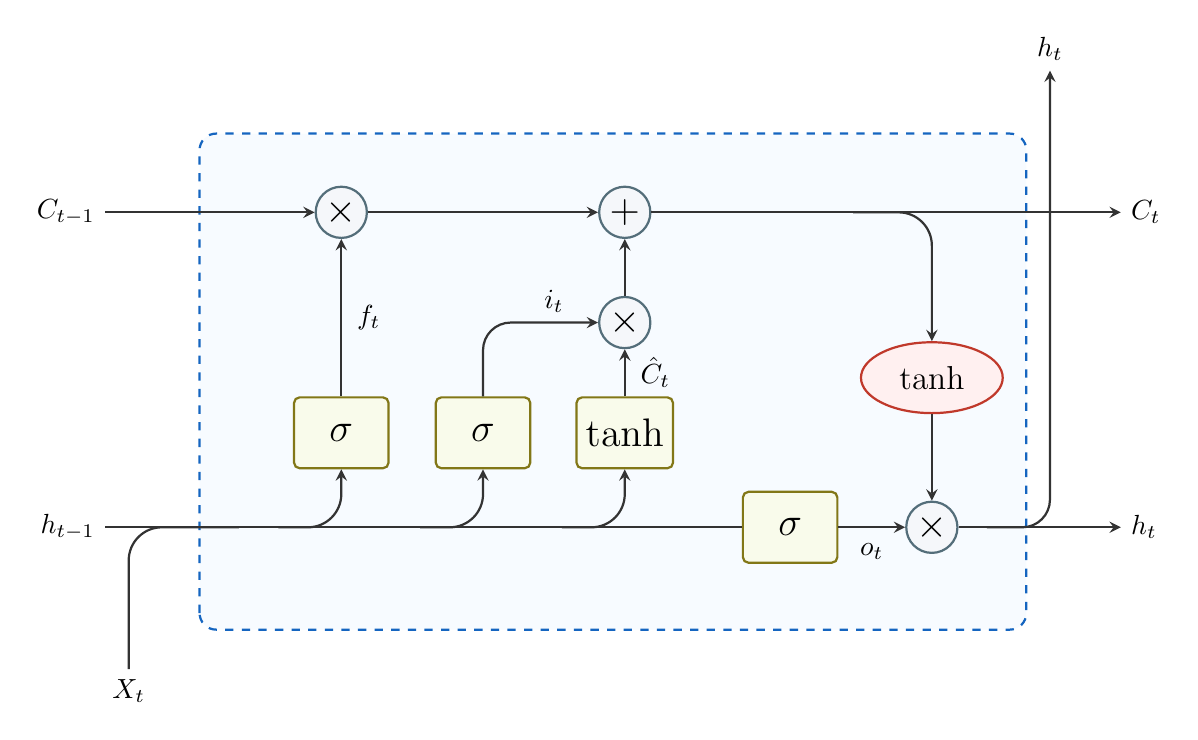
\begin{tikzpicture}[
    >=stealth, % 与 arch.tex 一致的箭头风格
    font=\sffamily,
    % 定义组件样式 (与 arch.tex 风格统一)
    nnbox/.style={draw=boxdraw, fill=boxfill, thick, rounded corners=2pt, minimum width=1.2cm, minimum height=0.9cm, align=center, font=\Large},
    operator/.style={circle, draw=opdraw, fill=opfill, thick, minimum size=0.65cm, inner sep=0pt, font=\Large},
    nntanh/.style={ellipse, draw=nntanhdraw, fill=nntanhfill, thick, rounded corners=2pt, minimum width=1.8cm, minimum height=0.9cm, align=center, font=\large},
    arrow/.style={->, thick, draw=black!80, rounded corners=4pt},
    line/.style={-, thick, draw=black!80}
]

% 核心 Y 轴高度定义
\def\Cheight{5}    % 顶部 C 状态线高度
\def\Hheight{1}    % 底部 h 状态线高度

% ==========================================
% 1. 绘制背景区域 (与 arch.tex 一致的虚线边框风格)
% ==========================================
% 按照原图包裹范围，左侧留出输入线，右侧留出输出线，顶部低于 h_t 输出
\begin{scope}[on background layer]
    \filldraw[fill=bgfill!40, draw=bgdraw, thick, dashed, rounded corners=6pt]
        (1.0, -0.3) rectangle (11.5, 6.0);
\end{scope}

% ==========================================
% 2. 放置核心节点与操作符 (精准坐标定位)
% ==========================================
% 底部四个神经网络门控 (其中前三个悬浮，第四个压线)
\node[nnbox] (f_gate) at (2.8, 2.2) {$\sigma$};
\node[nnbox] (i_gate) at (4.6, 2.2) {$\sigma$};
\node[nnbox] (c_cand) at (6.4, 2.2) {$\tanh$};
\node[nnbox] (o_gate) at (8.5, \Hheight) {$\sigma$};

% C 状态线上的加乘操作
\node[operator] (op_f) at (2.8, \Cheight) {$\times$};
\node[operator] (op_c) at (6.4, \Cheight) {$+$};

% 内部的乘法操作与椭圆 tanh
\node[operator] (op_i)   at (6.4, 3.6) {$\times$};
\node[nntanh]   (tanh_c) at (10.3, 2.9) {$\tanh$};
\node[operator] (op_o)   at (10.3, \Hheight) {$\times$};

% ==========================================
% 3. 绘制主干线与直接连线
% ==========================================
% 顶部 C_{t-1} 到 C_t 主干线
\draw[arrow] (-0.2, \Cheight) node[left] {$C_{t-1}$} -- (op_f);
\draw[arrow] (op_f) -- (op_c);
\draw[arrow] (op_c) -- (12.7, \Cheight) node[right] {$C_t$};

% 底部 h_{t-1} 与 X_t 的合并主干线 (穿入 Output Gate)
\draw[line] (-0.2, \Hheight) node[left] {$h_{t-1}$} -- (o_gate.west);
% X_t 从底部切入主干线的弯曲 (完美还原原图左下的曲线切入)
\draw[line, rounded corners=12pt] (0.1, -0.8) node[below] {$X_t$} |- (1.5, \Hheight);

% ==========================================
% 4. 绘制分支线与内部连线 (严格还原直角+圆角转弯)
% ==========================================
% 从 h 主干线向上的三个分支 (利用 -| 语法生成重叠后向上的弯折)
\draw[arrow, rounded corners=12pt] (2.0, \Hheight) -| (f_gate.south);
\draw[arrow, rounded corners=12pt] (3.8, \Hheight) -| (i_gate.south);
\draw[arrow, rounded corners=12pt] (5.6, \Hheight) -| (c_cand.south);

% 门控的直接向上的输出
\draw[arrow] (f_gate.north) -- (op_f.south) node[midway, right=2pt] {$f_t$};
\draw[arrow] (c_cand.north) -- (op_i.south) node[midway, right=2pt] {$\hat{C}_t$};

% i_gate 的折线输出 (上 -> 右 -> 入乘法器)
\draw[arrow, rounded corners=10pt] (i_gate.north) |- (op_i.west);
\node[above] at (5.5, 3.6) {$i_t$}; % i_t 文本在横线上方

% 内部加法的汇合连线
\draw[arrow] (op_i.north) -- (op_c.south);

% 顶部 C 线分支进入右侧 tanh 椭圆 (右 -> 下 -> 入椭圆)
\draw[arrow, rounded corners=12pt] (9.3, \Cheight) -| (tanh_c.north);

% 椭圆 tanh 到下方乘法器
\draw[arrow] (tanh_c.south) -- (op_o.north);

% Output Gate (o_t) 到下方乘法器
\draw[arrow] (o_gate.east) -- (op_o.west) node[midway, below=2pt] {$o_t$};

% 最终 h_t 状态向右与向上的双输出
\draw[arrow] (op_o.east) -- (12.7, \Hheight) node[right] {$h_t$};
% 向上的 h_t (复刻原图先向右一小段再向上穿越背景框的动作)
\draw[arrow, rounded corners=10pt] (11.0, \Hheight) -| (11.8, 6.8) node[above] {$h_t$};

\end{tikzpicture}
\end{document}